Rope Skipping (RS) (Abb.:\ref{fig:Seilchenspringer}) has been a common leisure-time activity of children for generations \cite{gowitzke1989}. Today, especially Asia holds high popularity of rope skippers with 87.4\% of the Chinese youth participating in jump rope exercises at least once a week \cite{Li2013}. Defined as a repetitive vertical jump with both feet losing contact to the ground to allow rope rotation \cite{gowitzke1989}, RS can be performed both outdoors and indoors by using inexpensive equipment \cite{wong2004}.\\
\begin{figure} [h] \centering
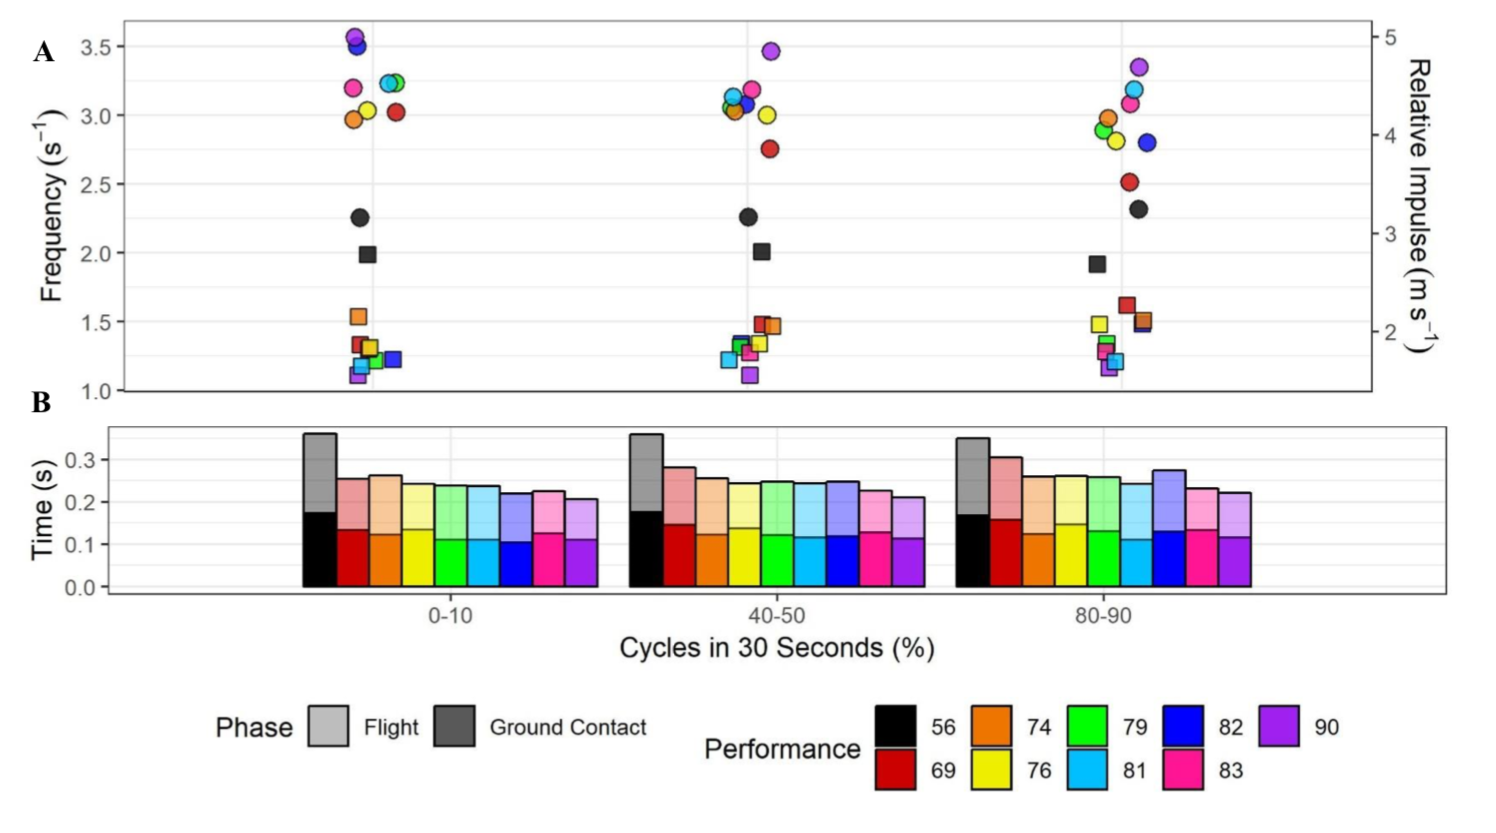
\includegraphics[width=0.9\textwidth]{pix/fig3.png}
    \caption{Hier steht dann die korrekte Beschreibung vom Bild manchmal sogar direkt mit einer Referenz \cite{Li2013}}
    \label{fig:Seilchenspringer}
\end{figure}
